% $Id: GMAT-Architectural-Specification.tex,v 1.34 2007/12/21 17:00:37 dconway Exp $
\documentclass[letterpaper,10pt]{book}

\usepackage[T1]{fontenc}
\usepackage[latin1]{inputenc}
\usepackage{geometry}
\usepackage{graphics,color}
\geometry{letterpaper}

% Enable indexing
\usepackage{makeidx}
\makeindex

%  for showing script lines as they appear in GMAT
\usepackage{verbatim}

% Allows alignment of multiple columns of text
\usepackage{array}

% Enables text wrapping around small tables and figures
\usepackage{float}

% Enables text wrapping around small tables and figures
\usepackage{floatflt}

% Enables side by side figures
\usepackage[countmax]{subfloat}

% Enables line numbering for verbatim text
\usepackage{lineno}

% Some text listing help for script files
\usepackage{listings}
\lstset{frame=single, captionpos=b, language=Matlab, xleftmargin=36pt, xrightmargin=36pt,
basicstyle=\ttfamily, numberstyle=\tiny, numbers=none}

% Use special characters defined by the ams
\usepackage{amsmath}

% Allow rotating figures
\usepackage{lscape}

% Enable verbatiminput so functional script files can be read in directly
\usepackage{fancyvrb}

% Fixes some font sizing problems
\usepackage{fix-cm}

%  for making index, using landscape mode, for multi page tables, supertabular??
% This package is needed to include the tables in the GMATDocuments/common subfolder
\usepackage{longtable, supertabular}

%\usepackage{rotating}  %This breaks the png files in \includegraphics{} calls???

% Used for table organization
\usepackage{tabularx}

%\usepackage[listofnumwidth=5.5em]{subfig}

% Used to customize table and figure list spacings
\usepackage{tocloft}

% Used to customize captions
\usepackage{caption}

% for creating bookmarks in the final pdf file when using dvipdfm
\usepackage[dvipdfm, bookmarks = true, bookmarksopen]{hyperref}

%% Used to build enumerations of the form 1.2.3.4.  etc.
%\usepackage[pointedenum]{paralist}

% If going through postscript to pdf, use the following instead for bookmarks:
%\usepackage[dvips, bookmarks = true, bookmarksopen]{hyperref}

%% Used to build the glossary and acronym definitions
%\usepackage[toc]{glossaries}

% Construct the basic page sizes
\oddsidemargin  0.0in
\evensidemargin 0.0in
\textwidth      6.5in
\headheight     0.25in
\topmargin      0.0in
\textheight=8.5in

% Note that png and jpg extensions are used for graphics
\DeclareGraphicsExtensions{.png,.jpg}

%% The following lines customize spacing on the tables of contents, list of figures, etc.
% More space for figure numbers
\setlength{\cftfignumwidth}{3em}
% Space between elements of the list
%\setlength{\cftbeforefigskip}{0.1cm}
% Space before chapter entries in the TOC
%\setlength{\cftbeforechapskip}{0.2cm}
% Space before parts in the TOC
%\setlength{\cftbeforepartskip}{0.7cm}

%\setlength{\emergencystretch}{6em}
%\pretolerance=10000
%\tolerance=10000

%\define@key{caption}{listofnumwidth}[4em]{\def\sf@numwidth{#1}}


%-------------------------------------------------------------------------------
%------------------------------------New Commands-------------------------------
%-------------------------------------------------------------------------------
\newcommand{\st}[1]{\begin{ttfamily}#1\end{ttfamily}}
\newcommand{\boldst}[1]{\begin{ttfamily}\textbf{#1} \end{ttfamily}}
\newcommand{\br}[0]{$\mathbf{r} $}
\newcommand{\bv}[0]{$\mathbf{v} $}
\newcommand{\ba}[0]{$\mathbf{a} $}
\newcommand{\mbr}[0]{\mathbf{r} }
\newcommand{\mbv}[0]{\mathbf{v} }
\newcommand{\mba}[0]{\mathbf{a} }

%-------------------------------------------------------------------------------
%------------------------------------New Environments---------------------------
%-------------------------------------------------------------------------------

\newenvironment{ScriptType}
  {\noindent \begin{ttfamily}}
   { \end{ttfamily} }

\newenvironment{Script}
 { \vspace{-.15 in} \begin{ttfamily} }
 { \end{ttfamily}\vspace{-.25 in} }

% Turned off the watermark for now because it's annoying in proof mode
% Make the watermark
\usepackage{eso-pic}
\usepackage{color}
\usepackage{type1cm}
%\makeatletter
%  \AddToShipoutPicture{%
%    \setlength{\@tempdimb}{.5\paperwidth}%
%    \setlength{\@tempdimc}{.5\paperheight}%
%    \setlength{\unitlength}{1pt}%
%    \put(\strip@pt\@tempdimb,\strip@pt\@tempdimc){%
%      \makebox(0,0){\rotatebox{45}{\textcolor[gray]{0.75}{\fontsize{2cm}{2cm}\selectfont{Draft:
%Work in Progress}}}}
%    }
%} \makeatother

% Disabled for intermediate versions -- TURN ON FOR RELEASE VERSIONS
%\makeatletter
%  \AddToShipoutPicture{%
%    \setlength{\@tempdimb}{.5\paperwidth}%
%    \setlength{\@tempdimc}{.5\paperheight}%
%    \setlength{\unitlength}{1pt}%
%    \put(\strip@pt\@tempdimb,\strip@pt\@tempdimc){%
%      \makebox(0,675){\rotatebox{0}{\textcolor[gray]{0.75}{\fontsize{1.5cm}{1.5cm}\selectfont{Draft:
% Work in Progress}}}}
%    }
%} \makeatother

% Not currently using glossaries package
%% Commands used to generate glossary and acronym tables
%\newglossary{definitions}{def}{dfn}{GMAT Nomenclature}
%\makeglossaries

% Float style for script files and snippets
\floatstyle{boxed}
\newfloat{script}{htb}{scr}[chapter]
\floatname{script}{Script}

\setcounter{secnumdepth}{3}

%-------------------------------------------------------------------------------
%------------------------------------Begin The Doc!!----------------------------
%-------------------------------------------------------------------------------
\begin{document}

%  Here we define the style for the bib.
\bibliographystyle{aiaa}
\thispagestyle{empty}

%%------------------------------------------------------------
%%-----------------Cover Page and TOC-------------------------
%%------------------------------------------------------------

\begin{center}
{\renewcommand{\thefootnote}{\fnsymbol{footnote}} { \Huge \bf
General Mission Analysis Tool\\ (GMAT)\\ Mathematical Specifications
}}
\end{center}
\begin{center}
{\renewcommand{\thefootnote}{\fnsymbol{footnote}} { \Huge \bf
 DRAFT }}
\end{center}

\begin{figure*}[htb]
\centering \centerline{
\begin{picture}(380,470)
\special{psfile= Images/GMATSplash.eps hoffset= 0 voffset= 0
hscale=60 vscale=60}
\end{picture}}
\end{figure*}
\vspace{-.2 in}
\begin{center}
\Large{NASA Goddard Space Flight Center\\
Greenbelt RD\\
Greenbelt, MD 20771}
\end{center}

\clearpage \clearpage


\tableofcontents

\chapter{Introduction}

This document contains a high level description of intended orbit
determination features for the General Mission Analysis Tool (GMAT).
The document contains two fundamental types of information:  how the
user would interact with GMAT to perform orbit determination, and a
high level view of how GMAT will solve orbit determination problems.
The user perspective is documented by discussing components in GMAT
that would  enable OD applications and through use cases that
suggest how components may be configured to solve common OD
problems.    The system perspective is documented by describing the
system components GMAT will employ to perform OD and how these
components interact including activity diagrams, sequence diagrams
and important classes and methods.

At the time of this writing, the General Mission Analysis Tool
(GMAT) does not support estimation of orbit or attitude related
data.   This document is the product of an intensive design session
performed at AFRL/RDSM in Maui with the goal to determine high level
user interface and architectural design specifications for new
estimation capabilities.   Our goals for the 8 day meeting were:

1)  Define high level functionality and detailed use cases 2)
Identify major system components:  objects, commands, and
application control 3)  Describe how components interact to solve
basic OD problems 4)  Identify priorities for development effort 5)
Continue development of prototype batch least squares functionality

Section 2 of this document  discusses how a user might interact with
GMAT to define and solve estimation problems.  This includes how to
configure estimators, how to define what quantities are to be
estimated and considered, and what measurements are to be included
in the estimation process.  For complex scenarios that involve
events, we propose a method for defining the event sequence so the
estimator can estimate their properties.  We also present an
approach for defining complex OD problems with smoothing and complex
measurement and solve for parameters.

Section three of this document is a system level perspective of how
identified features may be implemented in the system.  We identify
new system components and discuss how they interact to solve
estimation problems.    Finally, in section 4, we present a catalog
of use cases that describe the estimation problem to be solved and
illustrate how the user would configure GMAT to solve the problem.

\chapter{User Interfaces}
    \section{Overview and Philosophy}

    \section{Hardware Models}

\subsection{Receiver}

\subsection{Transmitter}

\subsection{Clock}

    \section{Measurement Models}

\subsection{Ground Station}

\subsection{GPS}

\subsection{TDRSS}

    \chapter{Solvers}  \label{Ch:Solvers}

\section{Differential Correction}

\section{Broyden's Method}

\section{Newton's Method}

\section{Matlab fmincon}

The user first creates a solver and names it.  An example is

 \st{ Create fminconOptimizer SPQfmincon}

 The user creates an optimization sequence by issuing an optimize
 command, followed by the name of the optimizer to use

 \st{Optimize SQPfmincon}

 \st{EndOptimize}

 \section{The Vary Command}
The user defines the independent variables by the vary command,

\begin{table}[htb]
\caption{ Available Commands in an fmincon Loop }
\begin{tabular}{p{1.5 in} p{1.5 in}}
   \hline
   Value & Command\\
   \hline \hline
     $X_i$ & \st{Vary} \\
    Upper Bound on $X_i$ & \st{Vary}  \\
   Lower Bound on $X_i$ & \st{Vary} \\
   Nondimensionalization Factor 1 & \st{Vary} \\
   Nondimensionalization Factor 2 & \st{Vary} \\
   Nonlinear constraint function& \st{NonLinearConstraint} \\
   Linear constraint function & \st{LinearConstraint} \\
   Cost Function & \st{OptimizerName.Cost = }\\
   \hline
 \end{tabular}
 \label{Table:EventFunction_dValues}
\end{table}

    \section{Estimation and Simulation}

    \section{Use Cases}

\subsection{Simple Batch Least Squares}

\subsection{Simple Extended Kalman Filter}

\subsection{Advanced SolverFor and Consider Parameters}

\subsection{Advanced Measurement Models}

\subsection{OD with Events}

\subsection{Measurement Simulation}

\subsection{Metric Calibration}

\subsection{Multiple Spacecraft Estimation}

\subsection{Non-Earth Estimation}


\chapter{Models and Mathematical Specifications}
    \section{OD State Vector}

\subsection{Spacecraft States}

\subsection{Dynamics Properties}

\subsection{Process Noise}

    \section{Propagation State Vector}

    \section{Estimators}

\subsection{Batch Least Squares}

\subsection{Extended Kalman Filter}

    \chapter{Measurement Classes and Measurement Models}

\chapauthor{Stephen P. Hughes}{NASA/Goddard Space Flight Center}
\chapauthor{Darrel J. Conway}{Thinking Systems, Inc.}
\chapauthor{Matthew P. Wilkins}{Schafer Corporation}

The Measurement classes define the interfaces used to work with measurement data during the estimation process.  These classes provide access to the observation data, typically provided by way of a data file, using a helper object derived from the MeasurementReader base class.  The Measurement classes provide methods that calculate the expected value of a specific measurement type, along with the derivative data needed for estimation.  These data include calculation of expected measurements, measurement partials, determination of measurement feasibility, and interactions with root finders to determine tracking schedules and light time corrections.  A measurement object acts as a participant in the measurement, as the measurement object contains estimated states associated with measurement errors.

The measurement hierarchy consists of a base class and a tiered hierarchy of derived classes as shown in Figure~\ref{fig:MeasurementClasses}.  The following sections discuss each class in the hierarchy in detail, starting with the Measurement base class.

\begin{figure}[htbp]
\begin{center}
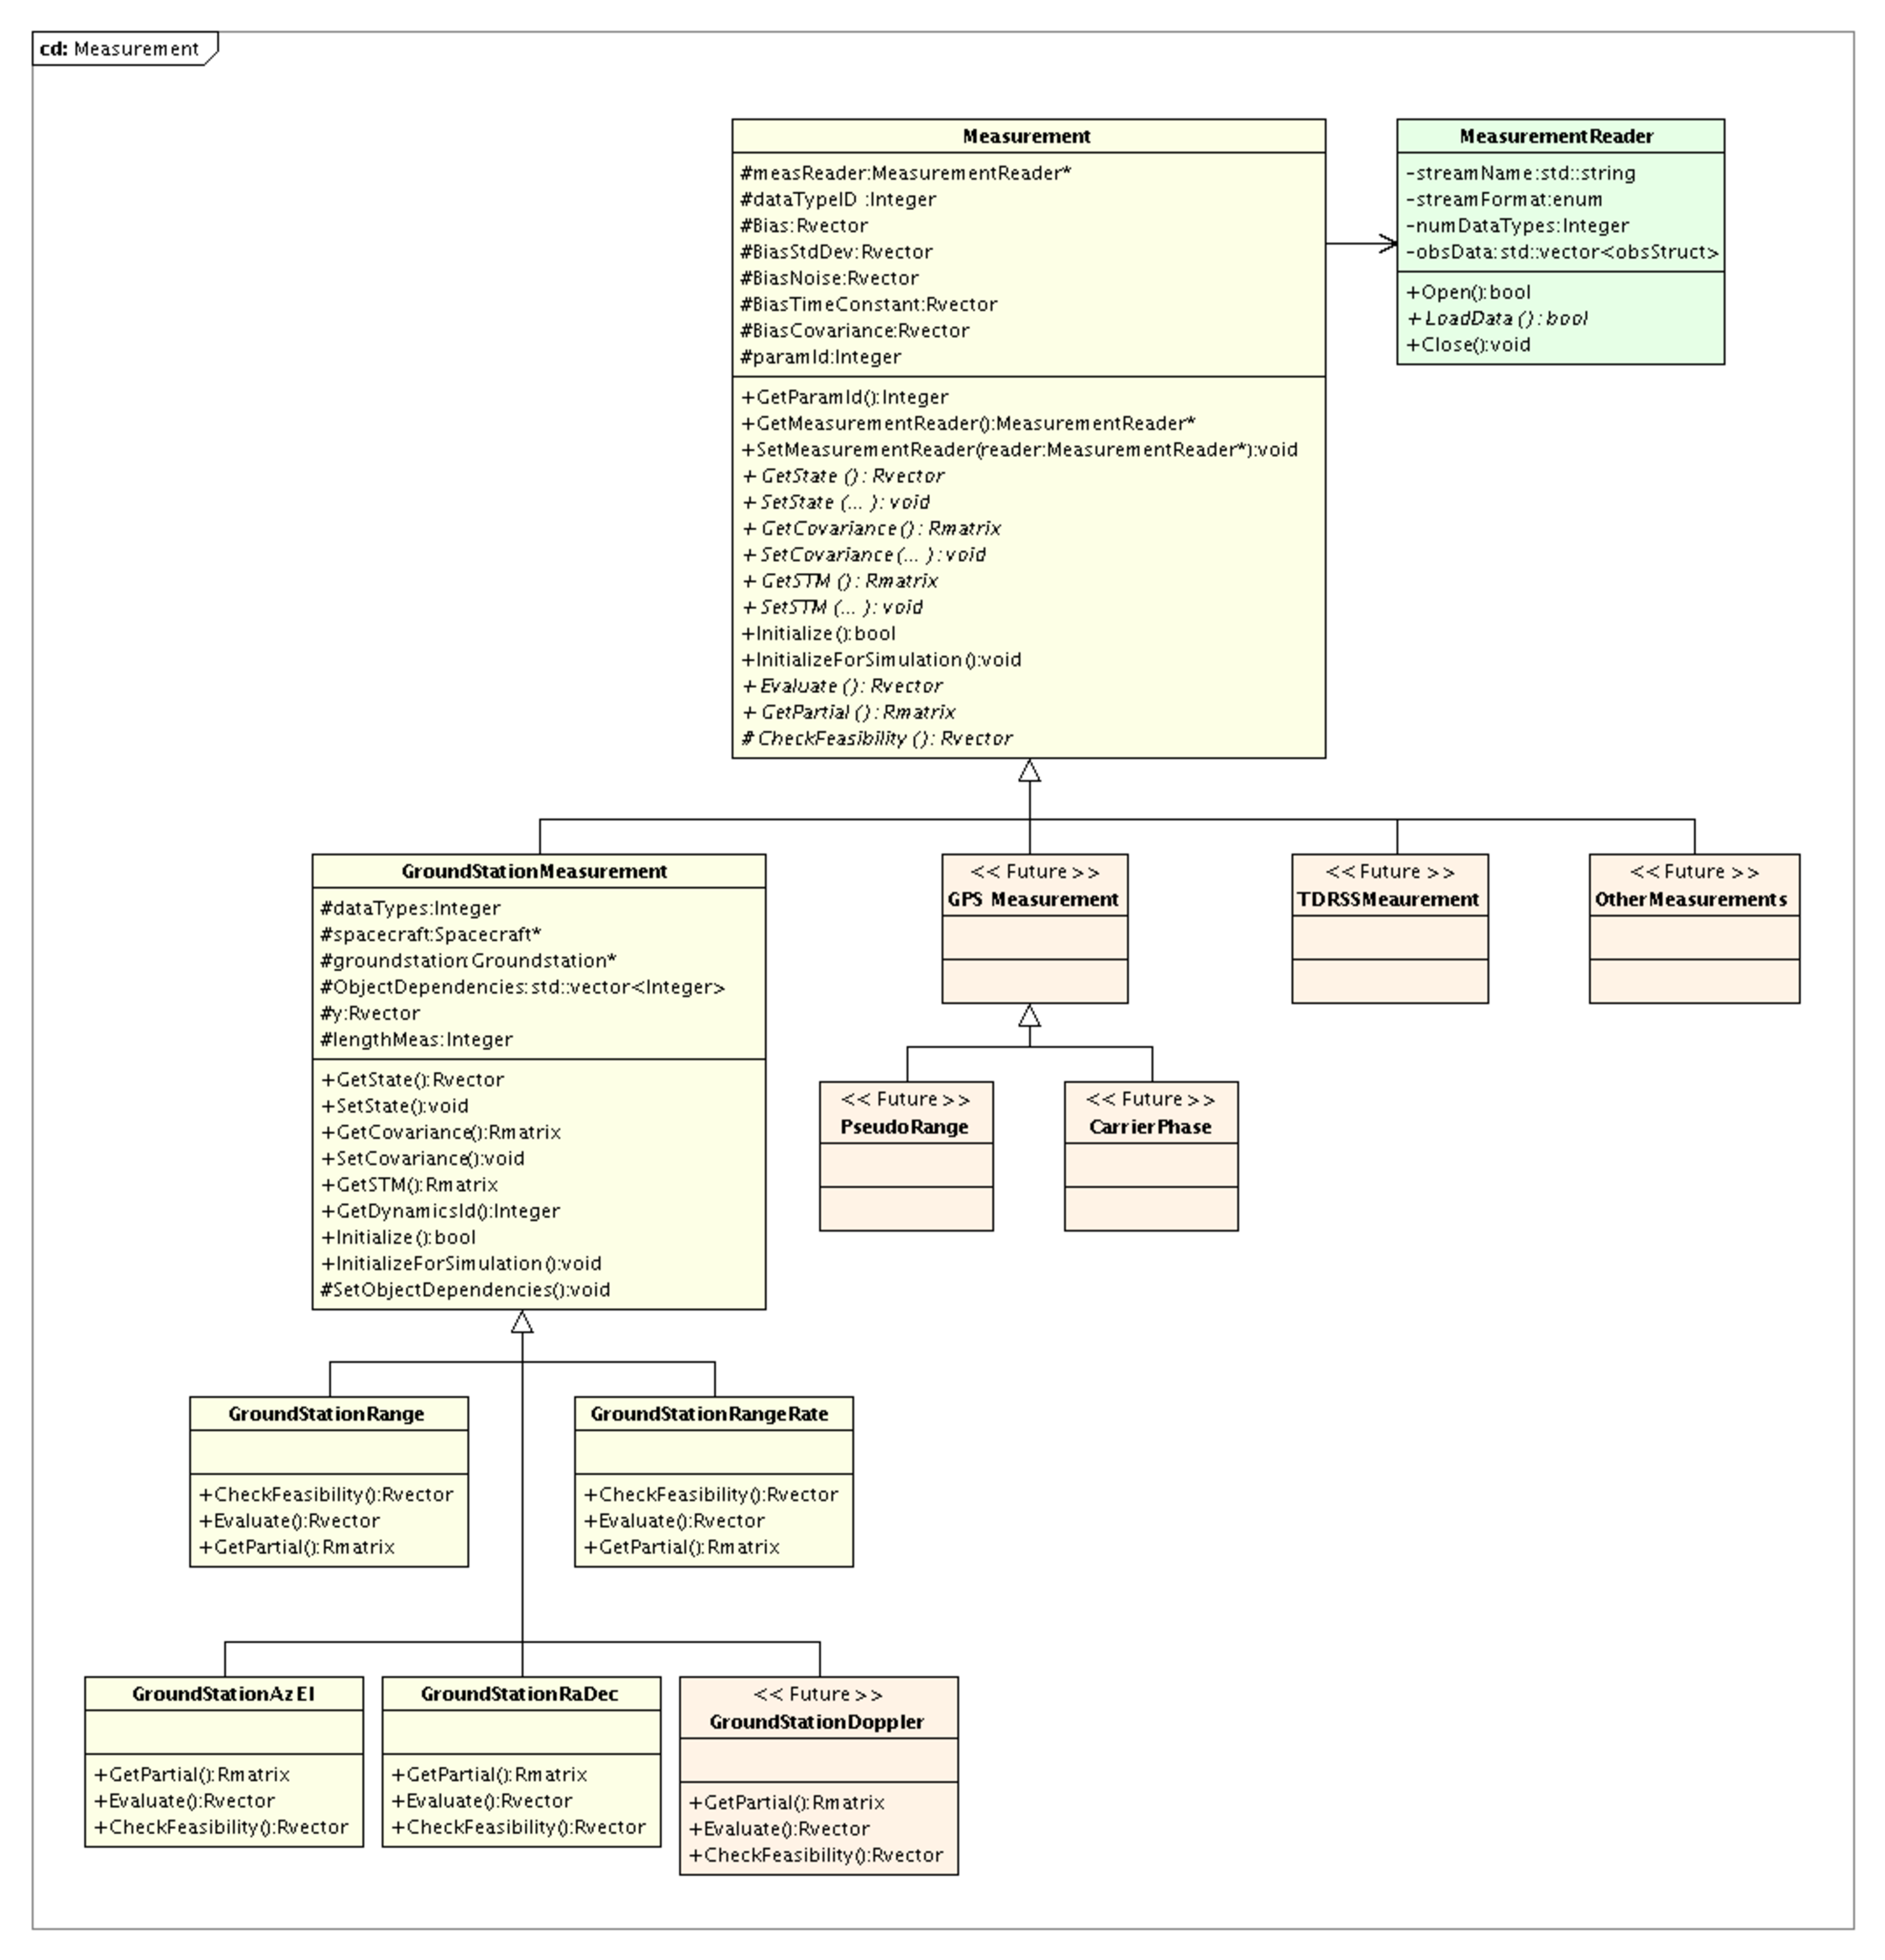
\includegraphics[scale=0.43]{Images/MeasurementClasses.eps}
% MeasurementClasses.png: 1061x1104 pixel, 72dpi, 37.43x38.95 cm, bb=0 0 1061 1104
\caption{\label{fig:MeasurementClasses}The Measurement Class Hierarchy}
\end{center}
\end{figure}

\section{The Measurement Class}

The Measurement base class contains member data and functions associated with all measurement objects as well as data associated with parameters that are set by the user when configuring the measurement object.  Examples of these data include the measurement file name and format, the data types to be processed from the file, and measurement stochastic properties such as biases and time constants.

The Measurement class defines many of the interfaces implemented in the derived classes so that the estimation process can work with measurement objects using base class references and pointers.  These interfaces are defined as either overridable or abstract (that is, pure virtual) methods on the Measurement base class.  The derived classes implement custom versions of these methods that are specific to the measurement type being implemented.  The data members of the Measurement base class are described below, followed by descriptions of the methods provided in the Measurement base class.  Finally, we will describe the MeasurementReader helper class before moving to the definitions of the derived classes.

\subsection{Measurement Members}

\paragraph{Member Attributes}

The list below describes the data elements provided in the Measurement base class to support the derived classes.  These elements are designed to facilitate access to measurement information through calls to a Measurement instance pointer.  Some Measurement objects provide multiple data elements.  For that reason, some of the data members listed here gain a dimension over what might be expected for single-valued measurements.  For example, the ground station RA/Dec measurement type returns two values for each measurement: the right ascension and declination values, so the methods that calculate these values return an Rvector rather than a Real number.  Since there are
Measurement classes that have this multivalued return requirement, GMAT uses an Rvector for the data, even when the return value is a single number.

The data members of the Measurement are:

\begin{itemize}
\item \textbf{MeasurementReader *measReader}:  The MeasurementReader that supplies the observation data. This pointer can be NULL when simulating data.
\item \textbf{Integer dataTypeID}:   An integer containing the Id for the data type.  Although the user may specify several data types on a measurement object, GMAT creates an object for each data type during initialization.  Each object has an Id associated with its data type which is specified by dataTypeId.
\item \textbf{Rvector Bias}:  A vector of real numbers containing the measurement biases.  These data can be estimation state parameters.
\item \textbf{Rvector BiasStdDev}:  A vector of real numbers containing the standard deviations of the biases. These data can be estimation state parameters.
\item \textbf{Rvector BiasNoise}:  A vector of real numbers containing the noise in the measurement biases. These data can be estimation state parameters.
\item \textbf{Rvector BiasTimeConstant}:  A vector of real numbers containing the time constants for the measurement biases. These data can be estimation state parameters.
\item \textbf{Rvector BiasCovariance}:  A vector of real numbers containing the bias covariances.
\item \textbf{Integer ParamId}:  ID for the type of measurement parameter?
\item \textbf{Integer numDataTypes}:  The number of data types the user specified on the measurement object. During measurement initialization, a new object is created for each data type specified on the measurement object.
\end{itemize}

\paragraph{Class Methods}

The Measurement class includes the following methods designed to make access to measurement data as generic as possible by the classes that use Measurement objects.  Many of these methods are abstract (pure virtual in C++ terminology): they are defined in this base class, but no implementation is provided in the base class.  The abstract classes can be identified by an ``= 0'' suffix in this list.

\begin{itemize}
\item \textbf{enum MeasurementFormat}: An enumeration defining the supported measurement formats.  Note: This enumeration is not a class member; it is a member of the Gmat namespace.
\item \textbf{Integer GetParameterId()}: A method to determine the integer id for solve-for and consider parameters on the measurement object.  This is how the system converts from the string definition provide by the user, say MauiGSRange.Bias,to a numeric Id.  <DJC: Not sure of this part.>
\item \textbf{MeasurementReader *GetMeasurementReader()}:  Retrieves a pointer to the
MeasurementReader.
\item \textbf{void SetMeasurementReader(MeasurementReader *reader)}:  Sets the pointer to the MeasurementReader.
\item \textbf{virtual Rvector\& GetState() = 0}: Retrieves the state vector.
\item \textbf{virtual void SetState(Rvector\& newState) = 0}:  Sets the state vector to match the provided data.
\item \textbf{virtual Rmatrix\& GetCovariance()= 0}:  Retrieves the covariance matrix.
\item \textbf{virtual void SetCovariance(Rmatrix\& newCovariance) = 0}:  Sets the covariance matrix data.
\item \textbf{virtual Rmatrix\& GetSTM() = 0}: Retrieves the state transition matrix.
\item \textbf{virtual void SetSTM(Rmatrix\& newSTM) = 0}: Sets the STM matrix data.
\item \textbf{virtual bool Initialize()}: Prepares the Measurement object for use in a Sandbox.
\item \textbf{virtual void InitializeForSimulation()}:  Prepares the Measurement object for use during measurement simulation.
\item \textbf{virtual Rvector\& Evaluate() = 0}:  Calculates the expected observation value.
\item \textbf{virtual Rmatrix\& GetPartial() = 0}:  Retrieves the measurement partial derivative matrix.
\item \textbf{virtual Rvector\& CheckFeasibility() = 0}:  Checks to see if a measurement can be made using the current state information.
\end{itemize}

\section{GroundstationMeasurement}

Measurements that are made at a ground station are modeled using the GroundStationMeasurement class.  Data and member functions that are common to all Ground Station measurements are located on the GroundStationMeasurement class, including the participants in the measurement process, Get/Set functions, and common modeling algorithms.   Below we discuss in detail all member data and functions.

\subsection{GroundstationMeasurement Members}

\paragraph{GroundStationMeasurent Attributes}

\begin{itemize}
\item \textbf{Integer dataTypes}:  ???
\item \textbf{Spacecraft *spacecraft}:  A pointer to the spacecraft that is participating in the measurement. This pointer is set during measurement initialization.
\item \textbf{Groundstation *groundstation}:  A pointer to the ground station that is participating in the measurement.  This pointer is set during measurement initialization.
\item \textbf{std::vector<Integer> ObjectDependencies}: A vector of integers that contains information on how participants on a measurement object map to participants in the overall estimation problem.  In general, the participants on a measurement are a subset of the participants for the estimation problem.  The ObjectDependencies is used primarily to determine partial derivatives and ensure they are placed in the correct location in the overall partial derivative array.  The ESM maintains an array of pointers, called ObjectsVector, to the participant associated with each state chunk in the estimation problem.  The ObjectDependencies array is the same length as ObjectsVector.  If, for example, element 1 of ObjectDependencies is zero, then the first object in the estimator's participant list is not a participant in the measurement.  If element 1 is nonzero, then the integer is associated with the participant Id used internally by the measurement.  The ObjectDependencies array is set during initialization when the Measurement Manager makes a call to initialize the measurement.
\item \textbf{Rvector y}:  The vector of calculated measurements.
\item \textbf{Integer lengthMeas}:  ???
\end{itemize}

\paragraph{}GroundStationMeasurement Methods:

\begin{itemize}
\item \textbf{SetState}:  Given a state value and id, this method updates the state on the measurement object.
\item \textbf{GetState}:  Given a state id, this method gets the state from the measurement object.
\item SetCovariance:  Given a covariance matrix and the state id, this method updates the state's covariance on the measurement object.
\item \textbf{GetCovariance}:  Given a state id, this method gets the state's covariance from the measurement object.
\item \textbf{GetSTM}: Given a state id, this method gets the states' STM.
\item \textbf{GetDynamicsId}:  Given a state Id, this method returns the ODE model ID for use in propagation of the state and it's STM.  Not implemented yet for measurement.
\item \textbf{Initialize}:  This method makes a call to the file reader and gets the observations and epochs from the requested data type.  If there are multiple data types on the measurement, the measurement object concatenates them into the Obs and Epochs Arrays.  These are then extracted by the measurement manager later in the initialization process.     For each data type, a new object is created and pointers to the object's participants are set.  (Matlab currently only supports one data type per measurement.  Not a difficult mod though)
\item \textbf{InitializeforSimulation}:  This method prepares a measurement object for simulation.  The process is similar to the Initialize method on GroundStationMeasurement, with the exception the reading and managing observations and epochs is not required.
\item \textbf{GetDataTypeId}:  This method returns the integer Id for the measurement type, given the string name for the measurement.
\item \textbf{SetObjectDependencies}:  This method takes as input an array of pointers to the participants in the estimation state vector.   The method steps through each element in the input array and determines if it points to any of the measurement participants.   If not, then the element in ObjectDependencies is set to zero.  If so, then the element is set to the Id of the participant used internally by the measurement object.
\end{itemize}

\section{GroundStationRange}

The GroundStationRange class is derived from the GroundStationMeasurement class, and performs modelling range measurements, measurement feasibility, and partial derivatives, and light time iteration.

\subsection{GroundstationRange Members}

\paragraph{GroundStationRange Attributes}

None.  The data members in the GroundStationMeasurement class are sufficient for this class.

\paragraph{GroundStationRange Methods}

\begin{itemize}
\item \textbf{CheckFeasibility}:  This method evaluates the feasibility function for the range measurement. If the value of the feasibility function is positive, then the conditions required to perform a measurement are met.  If the feasibility function is negative, conditions are not met.  Event locators determine the roots of the feasibility function to determine tracking data scheduling.
\item \textbf{Evaluate}:  The evaluate function calculate the computed value of the measurement based on the current state of the participants.
\item \textbf{GetPartial}:  This method returns the requested partial derivative based given a participant Id and the state Id.  The participant Ids are contained in the array ObjectDependencies.  This method is called by the measurement manager to determine individual partials. The measurement manager assembles the entire partial derivative from the pieces returned by the measurement object.
\end{itemize}

\section{The MeasurementManager Class}

The measurement manager functions as the interface between the Estimator and the measurement objects
defined by the user.  The primary jobs of the measurement manager are

\begin{itemize}
\item To coordinate measurement data and provide observed and computed values to the estimator
\item To maintain the sorted list of observed measurement quantities from all measurement sources.
\item To assemble the H matrix for each measurement based on state information and the partials map
provided by the measurements.
\end{itemize}


\chapter{High-level Architectural Design}
    \section{ OD State Vector }

    \section{Propagation State Vector } 

    \section{Estimators}

    \section{Measurement Processing}

    % $Id: Commands.tex,v 1.2 2008/02/16 00:54:59 dconway Exp $
\chapter{\label{chapter:Commands}Mission Control Sequence Commands}
\chapauthor{Darrel J. Conway}{Thinking Systems, Inc.}

\section{Command Overview}

Users model the evolution of spacecraft over time in GMAT using a mission control sequence that
consists of a series of commands.  These commands are used to propagate the spacecraft, model
impulsive maneuvers, turn thrusters on and off, make decisions about how the mission should evolve,
tune parameters, and perform other tasks required to perform mission analysis.  This chapter
describes the core components of the system that implement this functionality.
Chapter~\ref{chapter:SpecificCommands} provides a more in depth examination of the specific commands
implemented in GMAT, providing details about the implementation of each.

\section{Structure of the Sequence}

The mission control sequence is designed to present users with a configurable, flexible mechanism
for controlling the GMAT model.  Commands may manipulate modeled components, control model
visualization and other output data, determine the order of subsequent operations through looping or
branching, tune parameters to meet mission criteria, or group commands together to be executed as a
single block.  Each GMAT Sandbox is assigned its own mission control sequence\footnote{While the
current implementation of GMAT has a single Sandbox, GMAT is designed to support multiple
sandboxes.}.  This design feature drives the late binding features of objects in the GMAT Sandbox
(see Section~\ref{section:SandboxLateBinding}), which, in turn, places demands for late binding
support on the GMAT commands.  The following paragraphs provide an overview of these features.
Implementation details are described later in the chapter.

\subsection{Command Categories}
GMAT commands can be broken into four distinct categories: ``Regular'' commands, Control
Logic commands, Solver commands, and Function commands, as described here.

\paragraph{Regular commands} are commands that perform a single, isolated operation and do not
depend on any other command to operate.  Examples of the regular command are the Propagate command
and the Maneuver command.  The regular commands can appear anywhere in the Mission Control Sequence.

\paragraph{Control Logic commands} are used to perform control flow operations in the Mission
Control Sequence.  Each control logic command controls a list of commands -- called the command
subsequence -- that is executed by the control logic command when that command determines that
execution is needed.  All control logic commands are paired with a matching End command.  The End
commands identify the end of the command subsequence controlled by the control logic command.

GMAT supports three control logic commands: If, While and For, which are paired with the commands
EndIf, EndWhile and EndFor.  For commands are used to iterate over the subsequence for a fixed
number of iterations.  If commands provide a mechanism to fork the Mission Control Sequence based on
conditions detected during execution.  While commands are used to iterate over the command
subsequence until some condition is met.

\paragraph{Solver commands} are similar to control logic commands in that they manage a command
subsequence and use that subsequence to explore how changes in parameters affect the results of
executing the subsequence.  GMAT has three classes of solver commands: Targeters, Optimizers, and
Iterators.  Targeters adjust parameters in order to meet a specific set of goals.  Optimizers also
adjust parameters, in order to find the set that optimizes a problem objective.  Iterators are used
to observe the results of changes to parameters, so that the statistical behavior or the solution
space of the subsequence can be measured and recorded.

One key difference between solver commands and control logic commands is that for the control logic
commands, the changes to the spacecraft and other mission components applied during a subsequence
run affect subsequent runs of the subsequence.  Solvers reset the spacecraft states from one
iteration to the next, so that the effect of changes to the input parameters are applied to the same
set of initial conditions from one iteration of the subsequence to the next.

\paragraph{Functions} are used in GMAT to generalize common tasks, to communicate with MATLAB, and
to encapsulate multistep tasks into a single call in a mission.  \textit{The function subsystem
design will be documented at a later date.}

\subsection{Command Sequence Structure}

The mission control sequence is implemented as a linked list of command objects.  The sequence is
constructed from a script by appending links to the list as they are constructed by the script
interpreter.  Commands that control subsequences build the subsequences by managing a child linked
list.  The child list is constructed by appending links until the related subsequence termination
command is encountered, terminating the subsequence list.

Users can also interact with the command sequence from the GMAT GUI; these interactions let users
append commands to the sequence, insert commands at intermediate points, and remove commands.  Users
view the sequence as a hierarchical tree, as shown in Figure \ref{figure:HierarchicalMissionTree}.
The mission is modeled by executing the commands in the linked list sequentially.  The mission tree
shown on the GUI provides a graphical view into the linked list, including the command subsequences
for commands that control subsequences.  The top node in the tree is the the first link in the list;
in the figure, that node is a Propagate command, labeled Propagate1 on the mission tree.  The entire
linked list consists of seven nodes: Propagate - Propagate - Target - Propagate - Propagate - Target
- Propagate.  Each of the target nodes controls a subsequence used in the targeting process.  The
first of these nodes is expanded in the figure to show the subsequence.  For this example, the
subsequence consists of five links: Vary - Maneuver - Propagate - Achieve - EndTarget.

\begin{figure}[htb]
\begin{center}
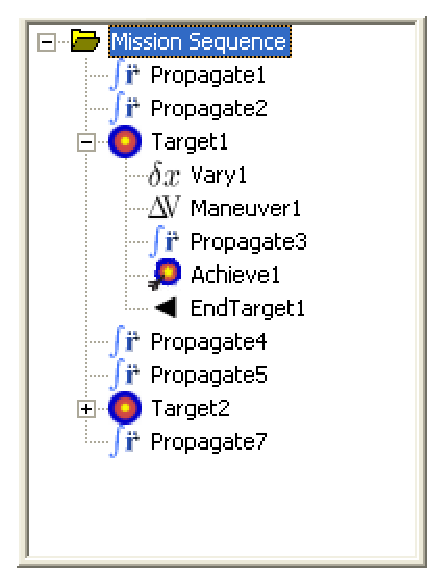
\includegraphics[scale=0.5]{Images/HierarchicalMissionTree.eps}
\caption{\label{figure:HierarchicalMissionTree}GMAT Command Sequence in the GUI}
\end{center}
\end{figure}

\textbf{Rework this piece -- it's not currently used} GMAT does not restrict the depth of the
nesting levels for the commands that control subsequences. The command classes include a counter
that monitors the current nesting level in the command sequence.  The nesting level is set when the
command is added to the linked list.  The main command sequence has a nesting level of 0.
Subsequences off of the main sequence increment the level to 1; subsequences contained in these
subsequences have a nesting level of 2, and so forth.  The subsequence termmination commands,
typically identified by an ``End'' prefix, have a nesting level set to the same level as the rest of
the subsequence, because they are the last command in the subsequence, and therefore exist at the
subsequence level.

\subsection{Command--Sandbox Interactions}

When a mission control sequence is run, all of the configured objects used in the run are copied
from the Configuration Manager into the Sandbox used for the run.  These copies are place into a
standard template library (STL) map matching the object names to pointers to the local copies in
the Sandbox.  These pointers need to be bound to the commands prior to execution of the mission
control sequence.  This late binding is performed during the initialization phase described below.
Additional details about the late bindign strategy implemented in GMAT can be found in
Section~\ref{section:SandboxLateBinding}.

During mission control sequence execution, the commands interact with the object copies to model
the interactions dictated for the model, as described in the execution section below.  These
interactions change the local copies, modeling the evolution of the system.  Once the command
sequence completes execution (either by finishing the sequence, encountering a ``Stop'' command, or
detecting a user generated stop event), each GMAT command is given the opportunity to complete any
pending operations.  This final step, described in the Finalization section below, is used to close
open file handles, clean up temporarily allocated memory, and perform any other housekeeping tasks
needed to maintain the mission control sequence for subsequent user actions.

\section{The Command Base Classes}

Figure~\ref{figure:CommandBaseClasses} shows core properties of the base classes used in the Command
subsystem.  The top level base class, GmatCommand, provides linked list interfaces and methods used
to parse command scripts.  BranchCommand adds capabilities to implement and execute commands that
run subsequences -- specifically, the Control Logic, Solver, and Function categories of commands.
Additional capabilities required by the Control Logic commands are provided by the ConditionalBranch
class.  Capabilities shared by all Solvers are implemented in the SolverBranchCommand class.

\begin{figure}
\begin{center}
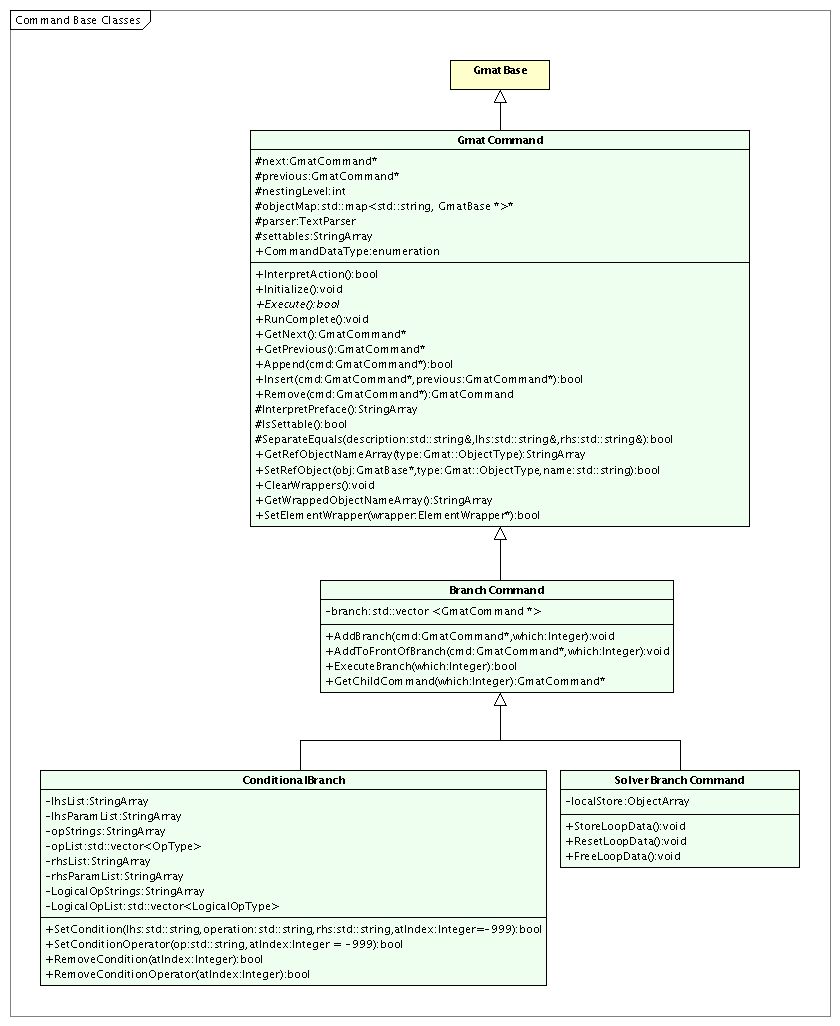
\includegraphics[scale=0.5]{Images/CommandBaseClasses.eps}
\caption{\label{figure:CommandBaseClasses}Base Classes in the Command Subsystem}
\end{center}
\end{figure}

\subsection{List Interfaces}

\textit{To be filled in}

\subsection{Object Interfaces}

\textit{To be filled in}

\subsection{Other Interfaces}

\textit{To be filled in}

\section{Script Interfaces}

The standard script syntax for a command is the command name followed by zero or more text strings
separated by white space.  Commands that are scripted using this syntax are handled generically in
the Interpreter subsystem, as described in Chapter~\ref{chapter:ScriptRW}\footnote{Some commands
that do not follow this generic description are also handled in the Interpreters at this writing.}.
Commands that use more complex scripting than a simple list of elements manage their own parsing in
a customized implementation of the InterpretAction() method.  This section describes the command
base class structures and methods that are used by commands that override InterpretAction() and
parse their configurations internally.  Parsing for Commands that do not override the
InterpretAction() method is handled in the ScriptInterpreter.  The methods described in the
following text are not used by those Commands.

\subsection{\label{section:ParametersInCommands}Data Elements in Commands}

Commands can be scripted to describe the actions taken on elements of the model (i.e. objects
instantiating GMAT classes), or to manipulate specific data elements of these objects based on the
rules encoded into the command.  When performing the latter task, the specific data element is
accessed using an ElementWrapper helper object that can manipulate data represented by the
following types: numbers, object properties, variables, array elements, and Parameter objects.  In
addition, commands may be construsted in the future that operate on Array objects and strings; the
infrastructure needed for these objects is included in the wrapper enumerations, but not yet
implemented.

The data wrappers are described in Section~\ref{section:DataWrappers}\footnote{The ElementWrappers
use the Adapter design pattern, described in \ref{section:TheAdapterPattern}}. These wrappers are
designed to be used by commands when needed to handle single valued Real data elements in the
commands.  The Gmat namespace includes an enumeration, WrapperDataType, with entries for each of the
supported data types.  This enumeration is described in Section~\ref{section:WrapperDataTypeEnum}.
The data wrappers are used to standardize the interface to numbers, object properties, variables,
array elements, and other Parameter objects to perform the command operations. Arrays and Strings
are handled separately by the commands -- arrays, because they can have more than one value, and
strings, because they do not provide Real number data for use in the commands.

\begin{figure}[htb]
\begin{center}
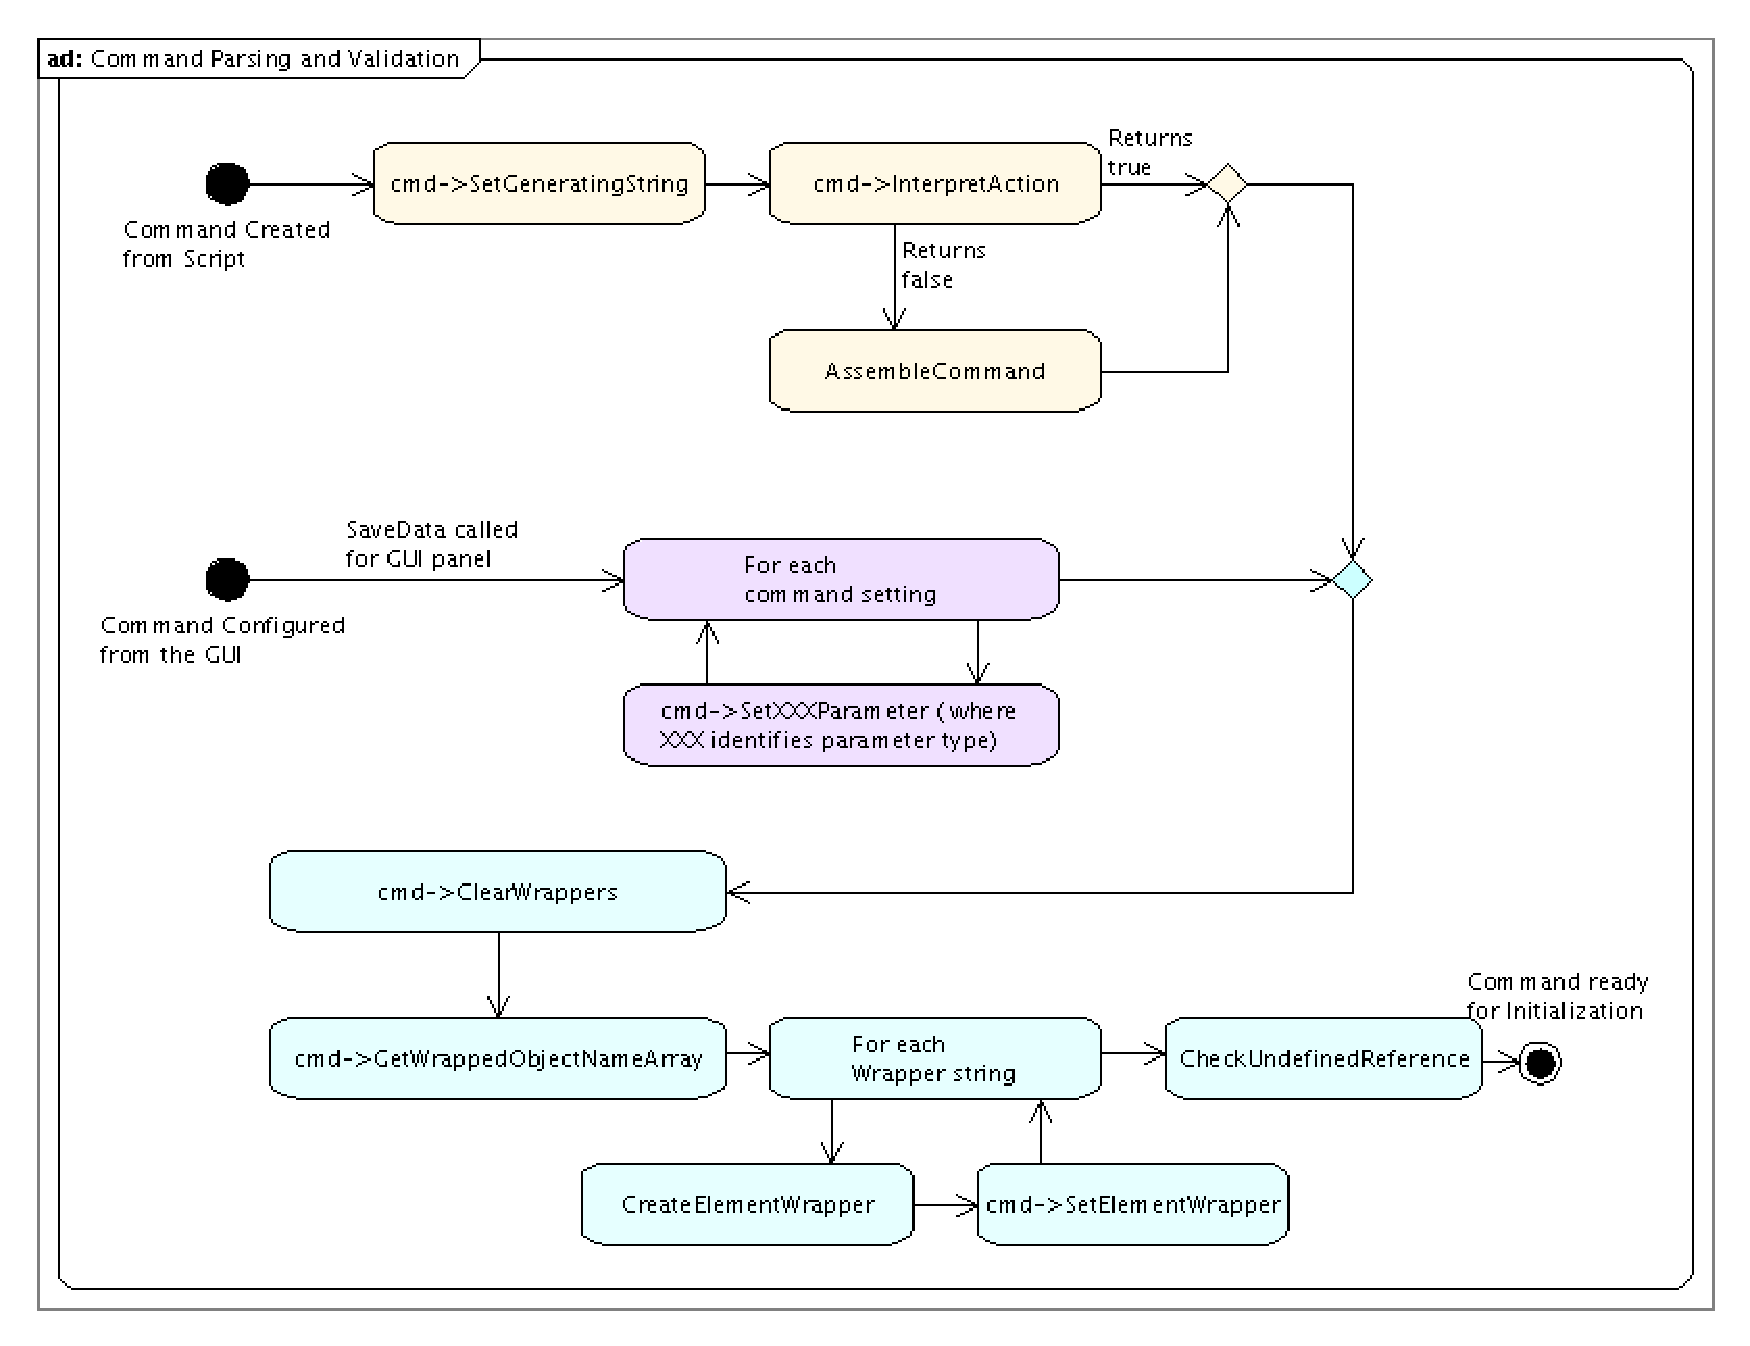
\includegraphics[scale=0.5]{Images/CommandParsingandValidation.eps}
\caption[Calls Made to Build and Validate Commands]{\label{figure:CommandParsingFlow}Calls Made in
the Interpreters to Build and Validate Commands.  Specific calls to the command are prefaced on this
diagram with the C++ pointer notation, ``cmd->''.}
\end{center}
\end{figure}

Figure~\ref{figure:CommandParsingFlow} shows an overview of the process used to build and validate
commands encountered in scripts and on the GUI.  The portions of the digram colored orange are
performed through calls launched by the ScriptInterpreter.  Commands created from the GUI follow the
procedure shown in purple.  In both cases, once the command has been built and the early binding
data has been set, the command is validated using methods provided by the Interpreter base class.
The calls made for this validation include calls that build the ElementWrapper members used in the
command.  These calls are shown in the figure in blue.

The process shown in Figure~\ref{figure:CommandParsingFlow} must be performed before the mission
control sequence can be executed in a Sandbox.  That includes identifying all of the names of
configured objects that the sequence will need, creation of any Parameters (performed in the
CheckUndefinedReference method) that will be required, and creation of the DataWrappers that will
need to be populated during Initialization in the Sandbox.

THe following subsections describe the support methods provided by the Interpreter and GUI
subsystems to configure the command objects.  These paragraphs are separated to match the three
sections of Figure~\ref{figure:CommandParsingFlow}.

\subsubsection{Scripted Command Configuration: Interpreter Support}

Scripted commands are configured using the Interpreter::CreateCommand method called from the
ScriptInterpreter while parsing a script.  The parsing process followed for commands is described
at a high level in Section~\ref{section:ParsingCommandBlocks}.  The Interpreter base class provides
several methods that facilitate that process, described here:

\begin{itemize}
\item \textbf{GmatCommand* CreateCommand(const std::string \&type, const std::string \&desc, bool
\&retFlag, GmatCommand *inCmd = NULL)}:  The method that drives the command creation process for the
ScriptInterpreter.  This method takes the generating string for the command as found in the script,
and creates an instance of the corresponding GmatCommand object.  It then calls InterpretAction() on
the command; if that call fails, it calls the Interpreter's AssembleCommand method.  Finally, it
builds any wrappers needed by the command, and validates that referenced objects used in the command
have been created.
\item \textbf{bool AssembleCommand(GmatCommand *cmd, const std::string \&desc)}:  Commands that are
not internally parsed are configured in this method.
\end{itemize}

Once this step has been completed, the command has been created and strings have been set decribing
all objects and data wrappers referenced by the command.  The data wrappers are not yet created;
thaqt process is described after the next subsection.

\subsubsection{Command Configuration in the GUI}

The GMAT GUI configures commands directly, based on the entries made by a user on the GUI panel
corresponding to the command.  Commands are created when a user inserts them into the mission
control sequence, configured with default settings.  When a user opens the configuration panel,
makes changes, and then applies the changes using either the Apply of OK button, the panel calls an
internal method, ``SaveData'', which passes the data on the panel to the command object.

The data passed into the object identifies all of teh objects referenced by the command.  Commands
configured by the GUI typically get populated with valid descriptors; as we will see shortly, the
 validation is repeated after the data wrappers are built, as described in teh next section.  All
data that requires wrappers is passed into the command as an std::string, using the
SetStringParameter method. The command stores these data for use contructing the wrappers.

\subsubsection{Interpreter Support for Wrappers and Validation}

Once GMAT has completed the steps described above, the command is configured with strings
describing wrappers and referenced objects, along with any other command specific data needed to
fully configure the command.  The final steps used configuring the command are shown in blue on
Figure~\ref{figure:CommandParsingFlow}.  These steps are all encapsulated in the Interpreter method
ValidateCommand.  The methods in the Interpreter base class used for wrapper construction and
validation are provided here:

\begin{itemize}
\item \textbf{void ValidateCommand(GmatCommand *cmd)}:  The method that executes the steps shown in
blue on the figure.  This method is called directly from the GUI, and as the final piece of
CreateCommand from the ScriptInterpreter.
\item \textbf{ElementWrapper* CreateElementWrapper(const std::string \&description)}:  This method
takes the descripion of a wrapper object and builds the corresponding wrapper.
\item \textbf{bool CheckUndefinedReference(GmatBase *obj, bool writeLine = true)}:  Method used to
verify that all referenced objects needed by the object (in this case, a Command) exist.  The
command is passed in as the first parameter.  The second parameter is a flag indicating if the line
number in the script should be written; for commands, that flag is left at its default true value.
\end{itemize}

\paragraph{CreateElementWrapper}  Of these methods, the CreateElementWrapper bears additional
explanation.  The following steps are implemented in that method:

\begin{enumerate}
\item Determine if the string is a number.  If so, create a NumberWrapper, set its value, and
return the wrapper.
\item Check to see if there a parentheses pair in the string.  If so, perform the following actions:
\begin{itemize}
\item Check to see if the text preceding the opening paren is an array.  If not, throw an exception.
\item Create an ArrayElementWrapper, and set the array name to the text preceding the opening paren.
\item Separate text enclised in the parentheses into row and column strings.
\item Call CreateElementWrapper() for the row and column strings, and set the corresponding
wrappers and strings in the ArrayElementWrapper.
\item Return the wrapper.
\end{itemize}
\item Check to see if there a period in the string.  If so, the wrapper needs to be either an
ObjectPropertyWrapper or a ParameterWrapper.  Performs these steps to create the correct type:
\begin{itemize}
\item Break apart the string using the GmatStringUtil::ParseParameter method.
\item Find the owner object, and check to see if it has the type provided in the string.  If so,
create an ObjectPropertyWrapper, otherwise create a ParameterWrapper
\item Set the description string.
\end{itemize}
Return the resulting wrapper.
\item Check to see if the string describes a Variable.  If so, create a VariableWrapper, set the
description and value, and return the wrapper; otherwise, throw an exception\footnote{A later build
will detect and return NULL for Array or String objects, so that they can be handled when needed.}.
\end{enumerate}

\subsection{Command Support for Parsing and Wrappers}

The command base class, GmatCommand, includes an instance of the TextParser described in
Section~\ref{section:TextParser}, along with an include statement for the GmatStringUtil namespace
definition (see Section~\ref{section:StringUtil} for details of the GmatStringUtil namespace).
These inclusions make all of the methods used for general purpose parsing of text from the
TextParser and the low level GmatStringUtil namespace functions available for use in command
parsing.  These elements are used by custom InterpretAction() methods when they are implemented for
the commands.

The base class also provides methods used during the creation and validation of the data wrappers.
These methods are used by the ScriptInterpreter, interacting with the Moderator in the
Interpreter::CreateCommand() method, to validate the objects required by the data wrappers.  The
methods supplied by the command base class to support data wrappers are described in
Section~\ref{section:CommandScriptingSupport}.  Before describing these methods, the wrapper
classes will be described.

\subsection{\label{section:DataWrappers}Data Type Wrapper
Classes\index{Wrappers}\index{Data Wrappers|see {Wrappers}}}

Many of the commands need to be able to treat all of the usable data types through a common
interface.  Table~\ref{table:ParameterInScriptExamples} presents representative examples to the
allowed data types in commands.  The data type interface used by the commands is captured in the
ElementWrapper class, shown with its subclasses in Figure~\ref{figure:CommandWrapperClasses}.
Derived classes are available for each of the supported types, using these classes:
NumberWrapper, ObjectPropertyWrapper, VariableWrapper, ArrayElementWrapper, and ParameterWrapper.
The Array class, when accessed as an entity rather than as a data provider for a single Real number,
is handled as a special case by any command designed to work with Array instances.  As indicated in
the table, no current command uses this capability, though it will be supported in the
NonlinearConstraint command in a future release of GMAT.  Similarly, strings are handled separately.

\begin{table}[tb]
\caption{\label{table:ParameterInScriptExamples}Script Examples of Parameters Used in Commands}
\begin{center}
\begin{tabularx}{6.3in}{|>{\raggedright\hspace{0pt}}p{1.1in}|>{\raggedright\hspace{0pt}}p{1.75in}
|X|}
\hline
\textbf{Type} & \textbf{Examples} & \textbf{Notes}
\tabularnewline \hline
Number & 1, 3.1415927, 3.986004415e5, 6.023e23 & Integers and Reals are treated identically
\tabularnewline \hline
Object Parameter & Sat.X, Burn.V, Thruster.ScaleFactor & Any object parameter
\tabularnewline \hline
Parameters & Sat.Longitude, Sat.Q4 & Any Calculated Parameter
\tabularnewline \hline
Variables & I, Var & Any Variable object
\tabularnewline \hline
Array Element & A(2,~3), B(I,~J), C(D(1,~K),~E(F(2,~3),~L)) & Any array entry.  Array row and
column indices can be specified using any allowed type
\tabularnewline \hline
Array & A & An entire array. Arrays are not yet supported in GMAT commands.  The
NonlinearConstraint command will be updated to use single column arrays (aka vectors) in a later
build.
\tabularnewline \hline
String & ``This is a string'' & A block of text treated as a single entity.
\tabularnewline \hline
\end{tabularx}
\end{center}
\end{table}

\begin{figure}[htb]
\begin{center}
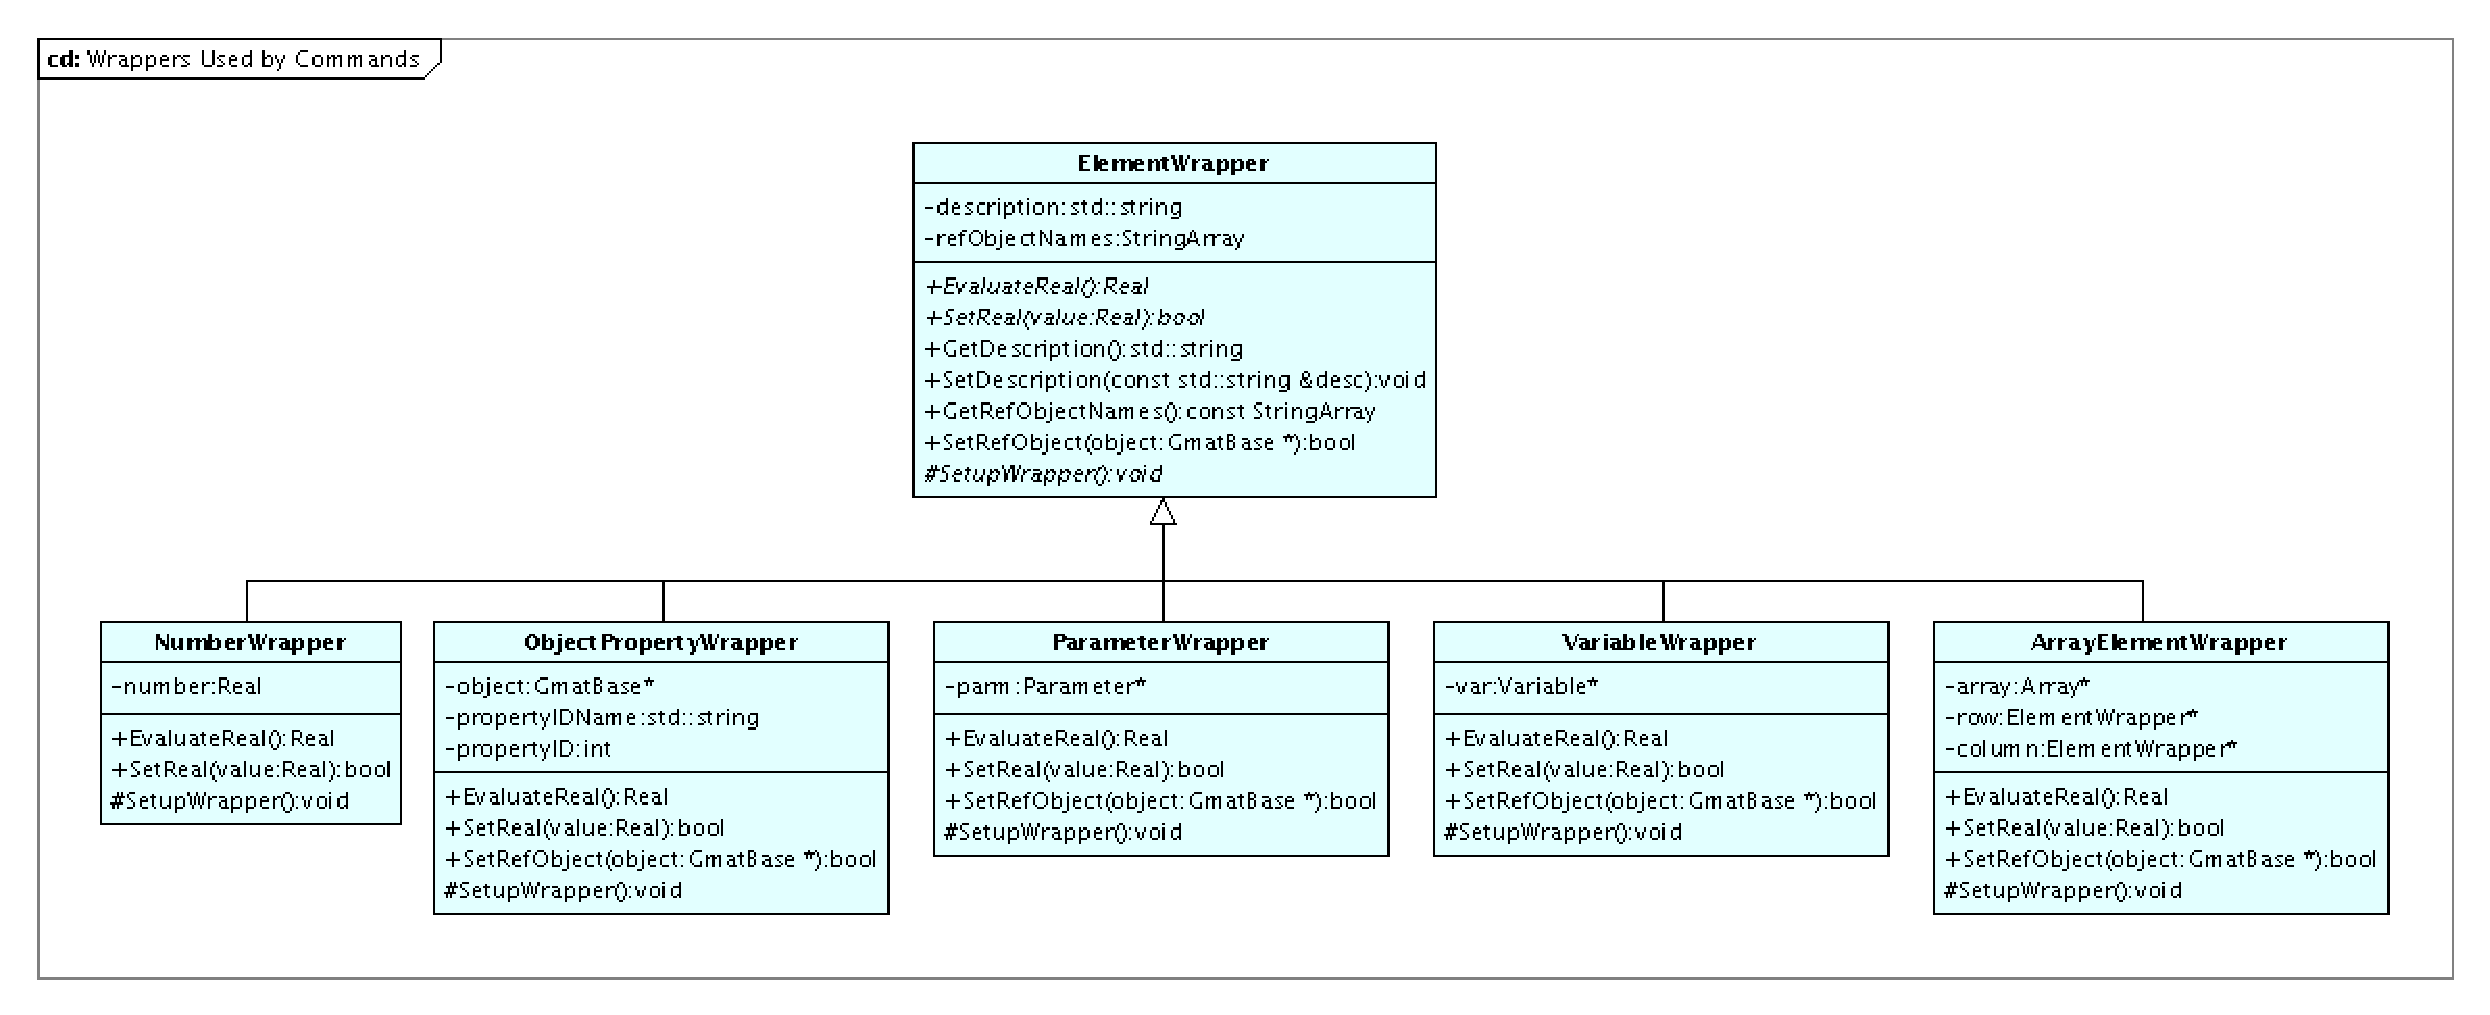
\includegraphics[scale=0.4]{Images/WrappersUsedbyCommands.eps}
\caption{\label{figure:CommandWrapperClasses}Parameter Wrappers Used by Commands}
\end{center}
\end{figure}

The wrapper classes implement the following methods:

\begin{itemize}
\item\textbf{std::string GetDescription()} Returns the current description string for the wrapper.
\item\textbf{void SetDescription(const std::string \&desc)} Sets the description string.
\item\textbf{const StringArray \&GetRefObjectNames()}: Returns a StringArray containing a list of
all reference objects used by the wrapper.
\item\textbf{bool SetRefObject(GmatBase *obj)}: Passes the a pointer to the reference object
into the wrapper so it can be assigned to the correct internal member.
\item\textbf{void SetupWrapper()}: Takes the description string and breaks it into components for
later use.
\end{itemize}

In addition, each ElementWrapper provides two abstract interfaces that can be used during command
execution:

\begin{itemize}
\item\textbf{Real EvaluateReal()} is used to calculate the current value of the wrapped
object, returning a Real number when fired.
\item\textbf{bool SetReal(const Real value)} takes a Real number as input, and sets the wrapped
element to that value.  It returns a flag indicating success or failure of the data setting
operation.
\end{itemize}

\noindent The derived wrapper classes implement these methods (and override the other methods as
needed) to access the data structures corresponding to each data type.

\subsection{\label{section:CommandScriptingSupport}Command Scripting Support Methods}

The Interpreter subsystem provides the methods needed to construct the data wrapper classes and
pass the wrappers into the commands.  GmatCommand provides the following methods to support this
process:

\begin{itemize}
\item\textbf{void ClearWrappers()}: Deletes all current wrappers in preparation for a new set of
wrapper instances.
\item\textbf{const Stringarray \&GetWrappedObjectNameArray()}: Returns a list of all wrapper
descriptions so that the required wrappers can be constructed.
\item\textbf{bool SetElementWrapper(ElementWrapper *wrapper)}: Sends the wrapper into the command.
If the wrapper is set correctly, this method returns true.  If the description contained in the
wrapper does not match a description in the command, the wrapper is destroyed, and false is returned
from this method.  All other error result in a thrown exception.
\end{itemize}

\noindent Note that commands own the wrappers passed in, and are responsible for managing the
associated memory.

\section{Executing the Sequence}

The mission control sequence is run in a GMAT Sandbox, following a series of steps described in
Section~\ref{section:SandboxMCSExecution}.  In this section, the command specific steps are
described in a bit more detail.

\subsection{Initialization}



\subsection{Execution}

\textit{To be filled in}

\subsection{Finalization}

\textit{To be filled in}

\subsection{Other Details}

\textit{To be filled in}



\end{document}

%------------------------------------------------------------
%-----------------Part I:  Mathematical Specifications-------
%------------------------------------------------------------
\chapter{Measurement Classes and Measurement Models}

\chapauthor{Stephen P. Hughes}{NASA/Goddard Space Flight Center}
\chapauthor{Darrel J. Conway}{Thinking Systems, Inc.}
\chapauthor{Matthew P. Wilkins}{Schafer Corporation}

The Measurement classes define the interfaces used to work with measurement data during the estimation process.  These classes provide access to the observation data, typically provided by way of a data file, using a helper object derived from the MeasurementReader base class.  The Measurement classes provide methods that calculate the expected value of a specific measurement type, along with the derivative data needed for estimation.  These data include calculation of expected measurements, measurement partials, determination of measurement feasibility, and interactions with root finders to determine tracking schedules and light time corrections.  A measurement object acts as a participant in the measurement, as the measurement object contains estimated states associated with measurement errors.

The measurement hierarchy consists of a base class and a tiered hierarchy of derived classes as shown in Figure~\ref{fig:MeasurementClasses}.  The following sections discuss each class in the hierarchy in detail, starting with the Measurement base class.

\begin{figure}[htbp]
\begin{center}
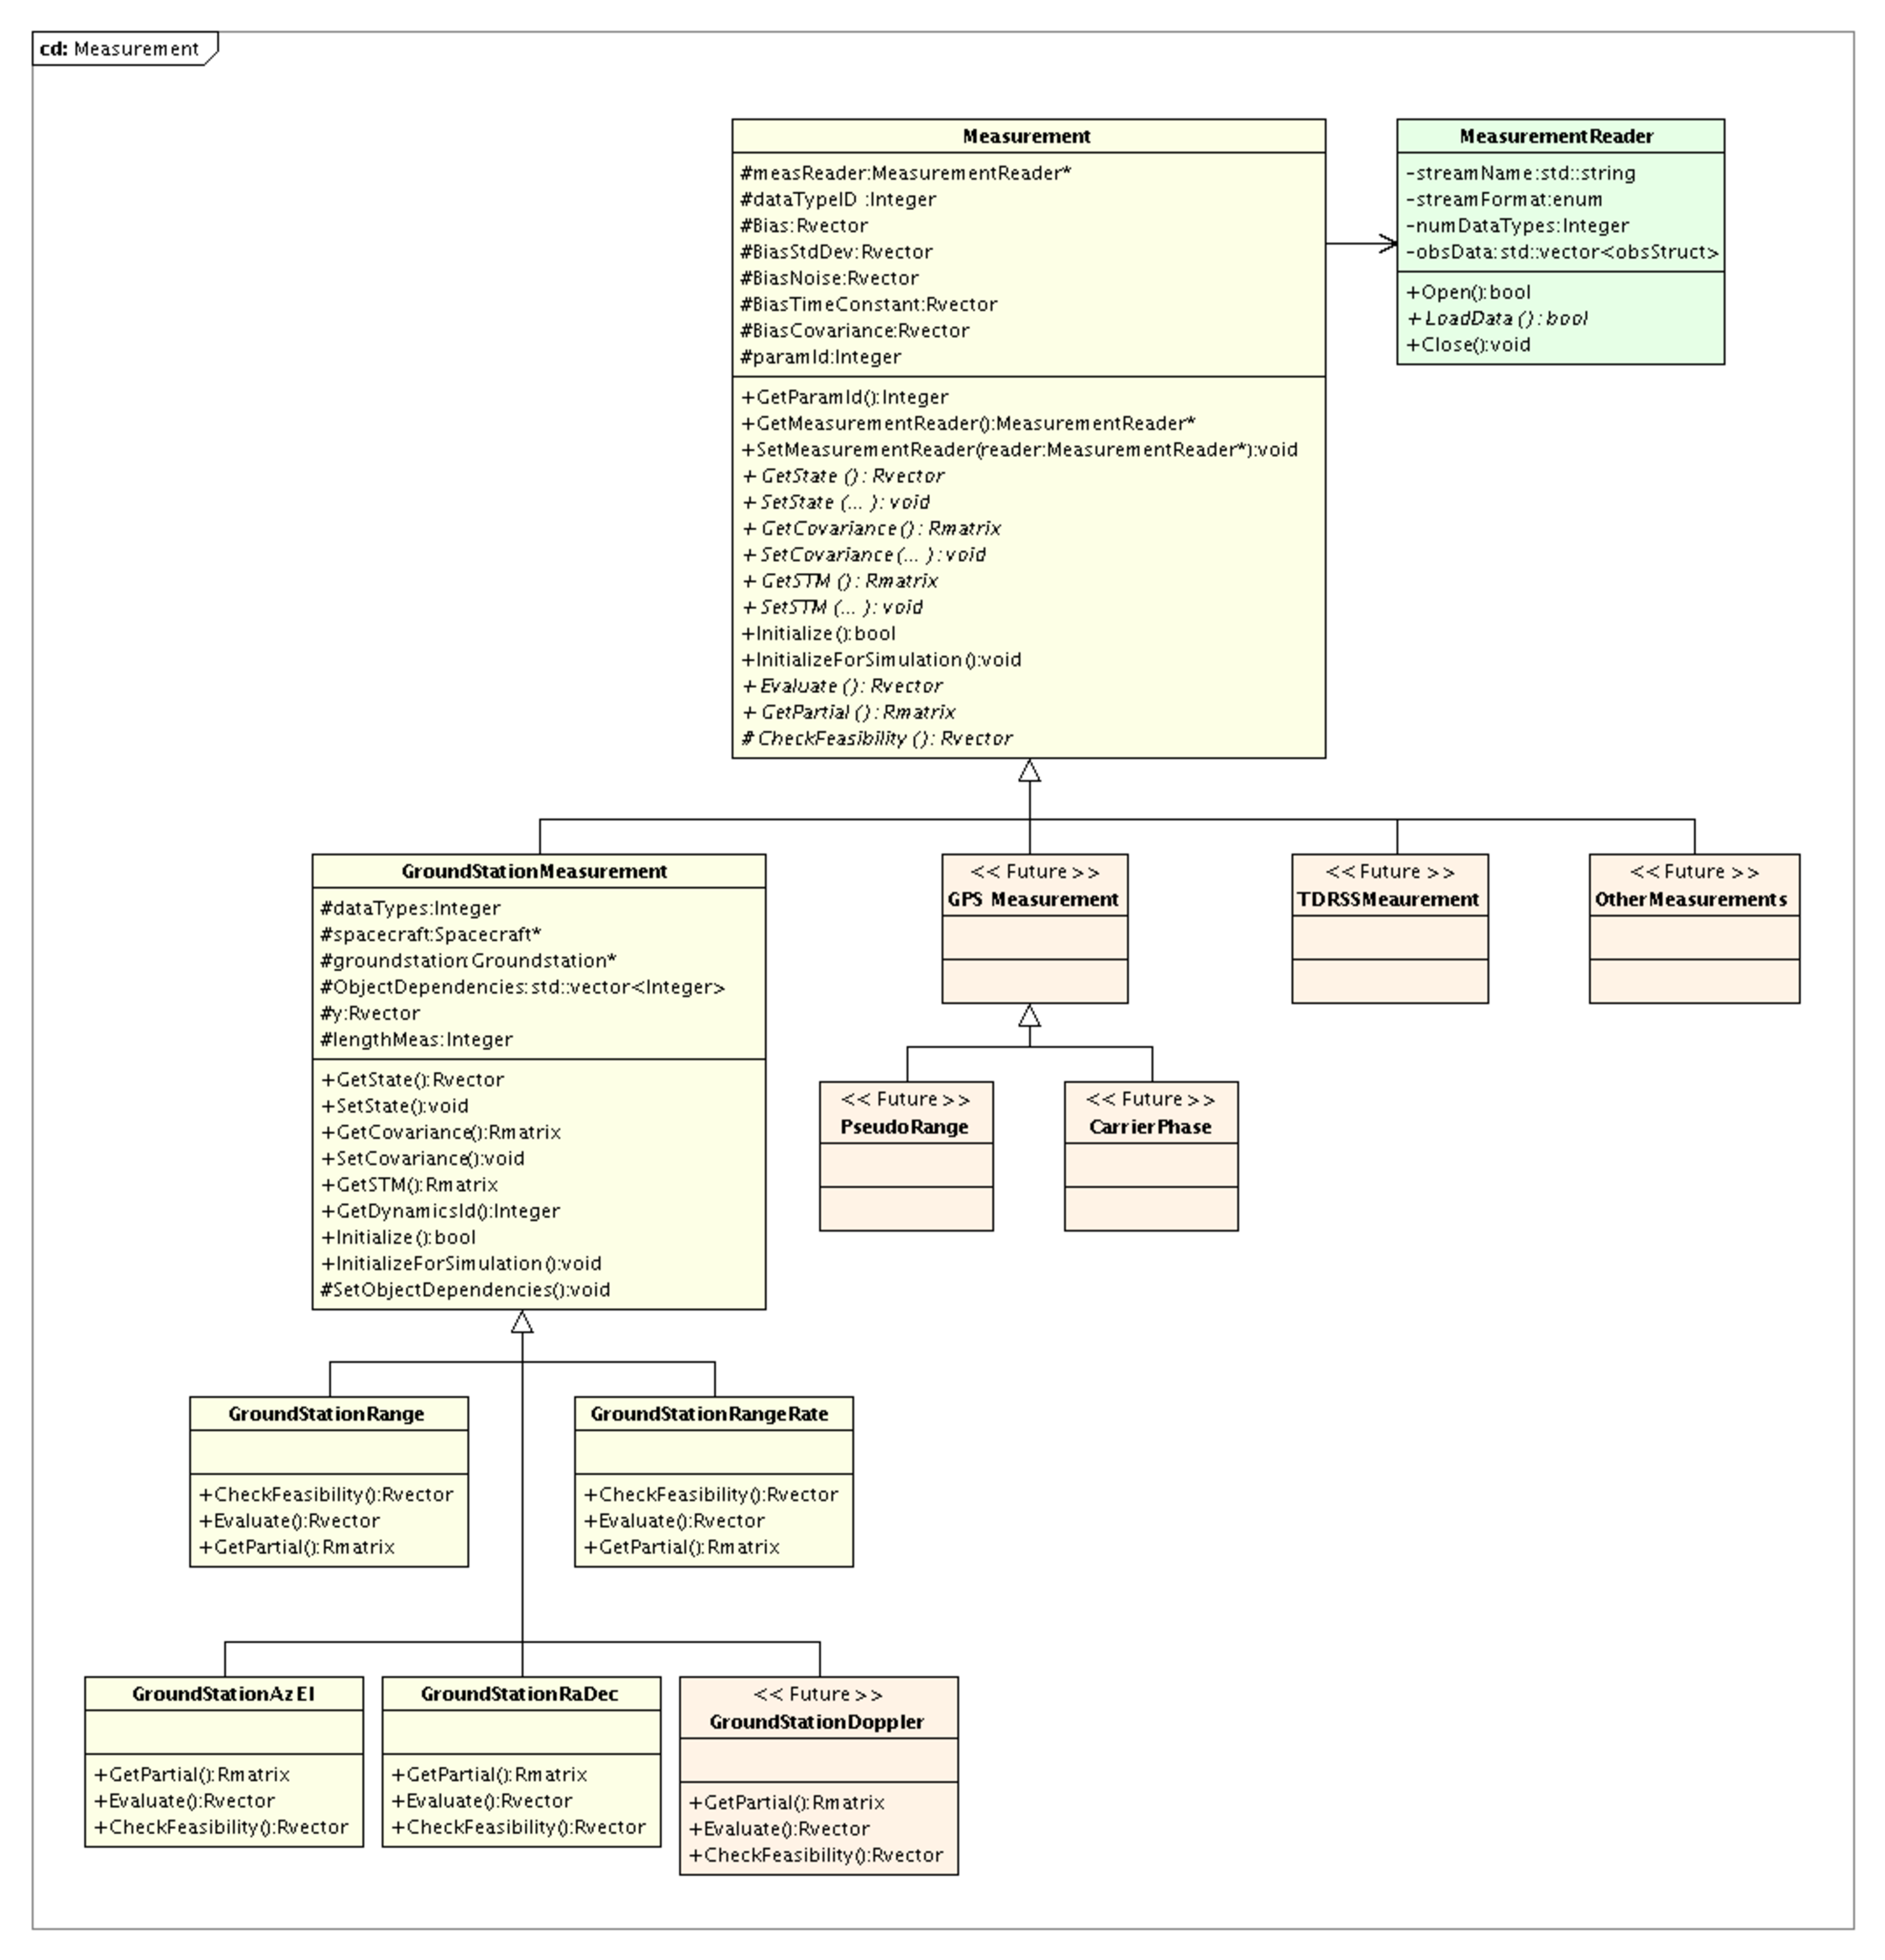
\includegraphics[scale=0.43]{Images/MeasurementClasses.eps}
% MeasurementClasses.png: 1061x1104 pixel, 72dpi, 37.43x38.95 cm, bb=0 0 1061 1104
\caption{\label{fig:MeasurementClasses}The Measurement Class Hierarchy}
\end{center}
\end{figure}

\section{The Measurement Class}

The Measurement base class contains member data and functions associated with all measurement objects as well as data associated with parameters that are set by the user when configuring the measurement object.  Examples of these data include the measurement file name and format, the data types to be processed from the file, and measurement stochastic properties such as biases and time constants.

The Measurement class defines many of the interfaces implemented in the derived classes so that the estimation process can work with measurement objects using base class references and pointers.  These interfaces are defined as either overridable or abstract (that is, pure virtual) methods on the Measurement base class.  The derived classes implement custom versions of these methods that are specific to the measurement type being implemented.  The data members of the Measurement base class are described below, followed by descriptions of the methods provided in the Measurement base class.  Finally, we will describe the MeasurementReader helper class before moving to the definitions of the derived classes.

\subsection{Measurement Members}

\paragraph{Member Attributes}

The list below describes the data elements provided in the Measurement base class to support the derived classes.  These elements are designed to facilitate access to measurement information through calls to a Measurement instance pointer.  Some Measurement objects provide multiple data elements.  For that reason, some of the data members listed here gain a dimension over what might be expected for single-valued measurements.  For example, the ground station RA/Dec measurement type returns two values for each measurement: the right ascension and declination values, so the methods that calculate these values return an Rvector rather than a Real number.  Since there are
Measurement classes that have this multivalued return requirement, GMAT uses an Rvector for the data, even when the return value is a single number.

The data members of the Measurement are:

\begin{itemize}
\item \textbf{MeasurementReader *measReader}:  The MeasurementReader that supplies the observation data. This pointer can be NULL when simulating data.
\item \textbf{Integer dataTypeID}:   An integer containing the Id for the data type.  Although the user may specify several data types on a measurement object, GMAT creates an object for each data type during initialization.  Each object has an Id associated with its data type which is specified by dataTypeId.
\item \textbf{Rvector Bias}:  A vector of real numbers containing the measurement biases.  These data can be estimation state parameters.
\item \textbf{Rvector BiasStdDev}:  A vector of real numbers containing the standard deviations of the biases. These data can be estimation state parameters.
\item \textbf{Rvector BiasNoise}:  A vector of real numbers containing the noise in the measurement biases. These data can be estimation state parameters.
\item \textbf{Rvector BiasTimeConstant}:  A vector of real numbers containing the time constants for the measurement biases. These data can be estimation state parameters.
\item \textbf{Rvector BiasCovariance}:  A vector of real numbers containing the bias covariances.
\item \textbf{Integer ParamId}:  ID for the type of measurement parameter?
\item \textbf{Integer numDataTypes}:  The number of data types the user specified on the measurement object. During measurement initialization, a new object is created for each data type specified on the measurement object.
\end{itemize}

\paragraph{Class Methods}

The Measurement class includes the following methods designed to make access to measurement data as generic as possible by the classes that use Measurement objects.  Many of these methods are abstract (pure virtual in C++ terminology): they are defined in this base class, but no implementation is provided in the base class.  The abstract classes can be identified by an ``= 0'' suffix in this list.

\begin{itemize}
\item \textbf{enum MeasurementFormat}: An enumeration defining the supported measurement formats.  Note: This enumeration is not a class member; it is a member of the Gmat namespace.
\item \textbf{Integer GetParameterId()}: A method to determine the integer id for solve-for and consider parameters on the measurement object.  This is how the system converts from the string definition provide by the user, say MauiGSRange.Bias,to a numeric Id.  <DJC: Not sure of this part.>
\item \textbf{MeasurementReader *GetMeasurementReader()}:  Retrieves a pointer to the
MeasurementReader.
\item \textbf{void SetMeasurementReader(MeasurementReader *reader)}:  Sets the pointer to the MeasurementReader.
\item \textbf{virtual Rvector\& GetState() = 0}: Retrieves the state vector.
\item \textbf{virtual void SetState(Rvector\& newState) = 0}:  Sets the state vector to match the provided data.
\item \textbf{virtual Rmatrix\& GetCovariance()= 0}:  Retrieves the covariance matrix.
\item \textbf{virtual void SetCovariance(Rmatrix\& newCovariance) = 0}:  Sets the covariance matrix data.
\item \textbf{virtual Rmatrix\& GetSTM() = 0}: Retrieves the state transition matrix.
\item \textbf{virtual void SetSTM(Rmatrix\& newSTM) = 0}: Sets the STM matrix data.
\item \textbf{virtual bool Initialize()}: Prepares the Measurement object for use in a Sandbox.
\item \textbf{virtual void InitializeForSimulation()}:  Prepares the Measurement object for use during measurement simulation.
\item \textbf{virtual Rvector\& Evaluate() = 0}:  Calculates the expected observation value.
\item \textbf{virtual Rmatrix\& GetPartial() = 0}:  Retrieves the measurement partial derivative matrix.
\item \textbf{virtual Rvector\& CheckFeasibility() = 0}:  Checks to see if a measurement can be made using the current state information.
\end{itemize}

\section{GroundstationMeasurement}

Measurements that are made at a ground station are modeled using the GroundStationMeasurement class.  Data and member functions that are common to all Ground Station measurements are located on the GroundStationMeasurement class, including the participants in the measurement process, Get/Set functions, and common modeling algorithms.   Below we discuss in detail all member data and functions.

\subsection{GroundstationMeasurement Members}

\paragraph{GroundStationMeasurent Attributes}

\begin{itemize}
\item \textbf{Integer dataTypes}:  ???
\item \textbf{Spacecraft *spacecraft}:  A pointer to the spacecraft that is participating in the measurement. This pointer is set during measurement initialization.
\item \textbf{Groundstation *groundstation}:  A pointer to the ground station that is participating in the measurement.  This pointer is set during measurement initialization.
\item \textbf{std::vector<Integer> ObjectDependencies}: A vector of integers that contains information on how participants on a measurement object map to participants in the overall estimation problem.  In general, the participants on a measurement are a subset of the participants for the estimation problem.  The ObjectDependencies is used primarily to determine partial derivatives and ensure they are placed in the correct location in the overall partial derivative array.  The ESM maintains an array of pointers, called ObjectsVector, to the participant associated with each state chunk in the estimation problem.  The ObjectDependencies array is the same length as ObjectsVector.  If, for example, element 1 of ObjectDependencies is zero, then the first object in the estimator's participant list is not a participant in the measurement.  If element 1 is nonzero, then the integer is associated with the participant Id used internally by the measurement.  The ObjectDependencies array is set during initialization when the Measurement Manager makes a call to initialize the measurement.
\item \textbf{Rvector y}:  The vector of calculated measurements.
\item \textbf{Integer lengthMeas}:  ???
\end{itemize}

\paragraph{}GroundStationMeasurement Methods:

\begin{itemize}
\item \textbf{SetState}:  Given a state value and id, this method updates the state on the measurement object.
\item \textbf{GetState}:  Given a state id, this method gets the state from the measurement object.
\item SetCovariance:  Given a covariance matrix and the state id, this method updates the state's covariance on the measurement object.
\item \textbf{GetCovariance}:  Given a state id, this method gets the state's covariance from the measurement object.
\item \textbf{GetSTM}: Given a state id, this method gets the states' STM.
\item \textbf{GetDynamicsId}:  Given a state Id, this method returns the ODE model ID for use in propagation of the state and it's STM.  Not implemented yet for measurement.
\item \textbf{Initialize}:  This method makes a call to the file reader and gets the observations and epochs from the requested data type.  If there are multiple data types on the measurement, the measurement object concatenates them into the Obs and Epochs Arrays.  These are then extracted by the measurement manager later in the initialization process.     For each data type, a new object is created and pointers to the object's participants are set.  (Matlab currently only supports one data type per measurement.  Not a difficult mod though)
\item \textbf{InitializeforSimulation}:  This method prepares a measurement object for simulation.  The process is similar to the Initialize method on GroundStationMeasurement, with the exception the reading and managing observations and epochs is not required.
\item \textbf{GetDataTypeId}:  This method returns the integer Id for the measurement type, given the string name for the measurement.
\item \textbf{SetObjectDependencies}:  This method takes as input an array of pointers to the participants in the estimation state vector.   The method steps through each element in the input array and determines if it points to any of the measurement participants.   If not, then the element in ObjectDependencies is set to zero.  If so, then the element is set to the Id of the participant used internally by the measurement object.
\end{itemize}

\section{GroundStationRange}

The GroundStationRange class is derived from the GroundStationMeasurement class, and performs modelling range measurements, measurement feasibility, and partial derivatives, and light time iteration.

\subsection{GroundstationRange Members}

\paragraph{GroundStationRange Attributes}

None.  The data members in the GroundStationMeasurement class are sufficient for this class.

\paragraph{GroundStationRange Methods}

\begin{itemize}
\item \textbf{CheckFeasibility}:  This method evaluates the feasibility function for the range measurement. If the value of the feasibility function is positive, then the conditions required to perform a measurement are met.  If the feasibility function is negative, conditions are not met.  Event locators determine the roots of the feasibility function to determine tracking data scheduling.
\item \textbf{Evaluate}:  The evaluate function calculate the computed value of the measurement based on the current state of the participants.
\item \textbf{GetPartial}:  This method returns the requested partial derivative based given a participant Id and the state Id.  The participant Ids are contained in the array ObjectDependencies.  This method is called by the measurement manager to determine individual partials. The measurement manager assembles the entire partial derivative from the pieces returned by the measurement object.
\end{itemize}

\section{The MeasurementManager Class}

The measurement manager functions as the interface between the Estimator and the measurement objects
defined by the user.  The primary jobs of the measurement manager are

\begin{itemize}
\item To coordinate measurement data and provide observed and computed values to the estimator
\item To maintain the sorted list of observed measurement quantities from all measurement sources.
\item To assemble the H matrix for each measurement based on state information and the partials map
provided by the measurements.
\end{itemize}


\end{document}
